% !TeX spellcheck = en_GB
%------------- PROG1P3 - REPORT -------------%
%--------------------------------------------%
%- @author Simon Bihel ----------------------% 
%- @author Florestan De Moor ----------------%
%- @version 1.0 -----------------------------%
%--------------------------------------------%

\documentclass[
	a4paper
]{article}

	\setlength{\parskip}{6mm plus2mm minus2mm}
	
\usepackage[english]{babel}

\usepackage[utf8]{inputenc}

\usepackage[T1]{fontenc} 

\usepackage[margin=2.5cm]{geometry}

\usepackage{graphicx}
	% Path of the pictures
	\graphicspath{{../src/main/resources/img/}{screens/}}

\usepackage{xspace}

\usepackage{amsmath}

\usepackage{amsfonts}

\usepackage{amssymb}

\usepackage{tikz}
	\usetikzlibrary{arrows}

\usepackage{xcolor,colortbl}

\usepackage{caption}

\usepackage{subcaption}
	
\usepackage{floatrow}	
	
\usepackage{float}



%% Specific commands %%
	\newcommand{\this}{\emph{Ant vs. SomeBees }}
	\newcommand{\theEnd}{\[\star ~ ~ ~ \star\]\[\star\]}


\begin{document}

\title{PROG1 P3 - Ant vs. SomeBees}
\author{Simon Bihel, Florestan De Moor \\ ENS Rennes, Computer Science Department, 1st year}
\date{December 13\(^{\text{th}}\), 2015}


\maketitle

\section*{Introduction} % To check, but seems ok

In this report, we present our work on the third project of the programming course. %
It consisted in creating a game based on the famous one \emph{Plants vs. Zombies$^\copyright$}. %
\this was programmed using the Scala language, and the Scala-swing library for the graphic interface. %
This project was done using mostly the OOP paradigm, but also some FP. %
First, we will introduce the game and its features. %
Then, we will expose the class diagram, and the structure we decided to use to create this game. %
Finally, we will clarify some parts of the implementation.


\section{Game overview} % To check, but seems ok

\this is a tower defence like game. The terms are really simple : the player controls an anthill, which has five tunnels. %
An army of bees will try to invade it. %
The goal is to survive as long as possible by killing the bees entering the tunnels in waves. %
If a bee succeed to go through a whole tunnel, the game is lost. %
Each bee killed gives the player 5 points, the player score is printed in the bottom information bar.

%
\begin{figure}[H]
	\foreach \x in {1,...,6} {
\includegraphics[scale=0.3]{tunnel.png}}
\includegraphics[scale=0.3]{tunnel_water.png}
	\caption{Example of tunnel}
	\label{tunnel}
\end{figure}
%

\paragraph{Defending the tunnels} In order to defend the tunnels, the player has the possibility to put some ants. %
This has a cost : food. The starting food amount is 2. The food amount is printed in the bottom bar. %
Each ant has specific cost, armour, and abilities. %
For example, the harvester ant collect 1 food per turn, while thrower ants can throw projectiles to attack bees. %
The bodyguard is a special unit, that can be put at the same place than another ant, in order to protect it.

%
\begin{figure}[H]
	\foreach \x in {harvester, fire, longthrower, scuba}{
	\includegraphics[scale=0.5]{ant_\x.png} }
	\caption{Some ants}
	\label{someants}
\end{figure}
%

\paragraph{Turns} The game is divided in turns. %
The bees are continuously moving at each frame, but actions such as food collecting or shooting are performed at each turn.

\paragraph{Bee waves} The first bee will come in after six turns, and one bee will appear at each turn from then on. %
The wave difficulty will increase : incoming bees will have greater armour, and damages up. %
There are two types of bees : the black ones, that can attack ants when they are right in front of them, and the red ones, that can shoot afar. %
A new bee appears in one of the five tunnels, picked up randomly.

%
\begin{figure}[H]
	
\includegraphics[scale=0.5]{bee.png}
	
\includegraphics[scale=0.5]{rangebee.png}
	\caption{Bees}
	\label{bees}
\end{figure}
%

\paragraph{Spells} The player has also the possibility to use spells. %
This also costs food. Three spells were implemented.
 
%
\begin{table}[H]
	\begin{tabular}{|c|p{13cm}|}
		\hline
		\rule[1mm]{0pt}{5mm}
		\raisebox{-.5\height}{
			
\includegraphics[scale=0.5]{freeze.png} }
		& The freeze ability can be applied on a place of the tunnel, and has for consequence to freeze all bees within for three turns. %
		Notice that they are unable to move, but not to shoot. \\
		\hline
		\rule[1mm]{0pt}{5mm}
		\raisebox{-.5\height}{
			
\includegraphics[scale=0.5]{radar.png} }
		 & The radar ability can be given to an ant. %
		 As long as the concerned ant is living, the player will be able to see the armour points of all bees in the specific tunnel. \\
		\hline
		\rule[1mm]{0pt}{5mm}
		\raisebox{-.5\height}{
			
\includegraphics[scale=0.5]{double.png} }
		 & The upgrade spell is very powerful : %
		 it can be applied to an ant, in order to level it up. %
		 This doubles its damage power. %
		 Notice that it doesn't modify armour points, the player has to protect well its upgraded ants. \\
		\hline
	\end{tabular}
	\caption{Spells implemented}
	\label{spellsTable}
\end{table}
%

\paragraph{GUI} The user interface contains a menu which allows the player to select a type of ant, or a spell. %
There is also a remove button, to delete existing ants. %
Notice that deleting an ant doesn't give back food. %
A message can be displayed in the bottom bar.

%
\begin{figure}[H]
	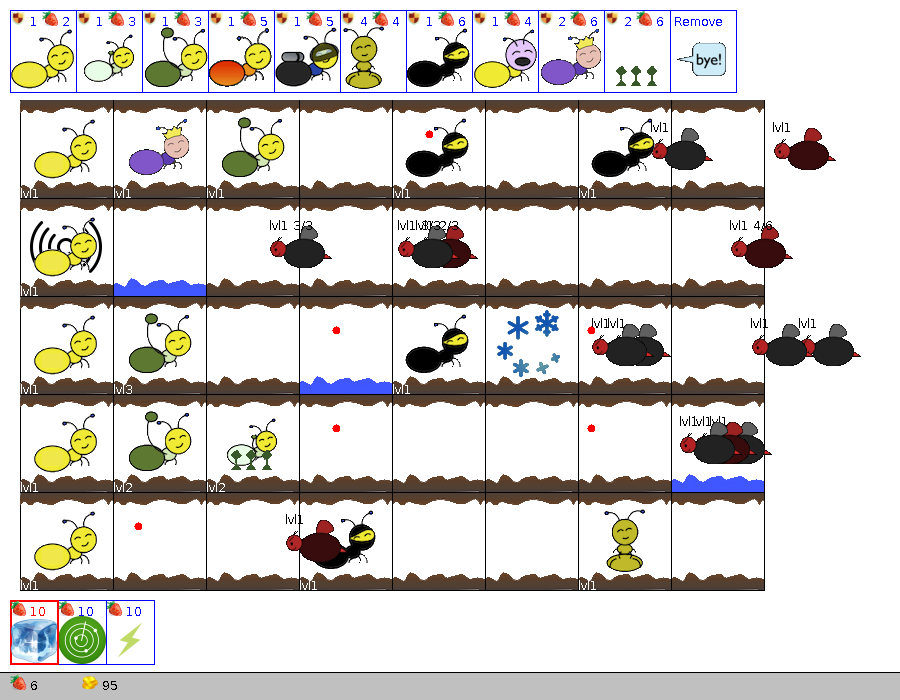
\includegraphics[scale=0.3]{screen2.png}
	\caption{Graphic User Interface}
	\label{gui}
\end{figure}
%


\section{Program's structure} % To develop more

The architecture of the program is based on a Model-View-Controller pattern. %
The View part displays the UI and warns the Controller of inputs. The Controller then decides what action should be done in response and asks the Model to do it. %
The latter, which only stores the elements of the game, executes the request. %
The game itself is composed of Places that contains Ants and Bees that fire Projectiles at each others. %
The overall interactions of the various parts of the program are shown in figure~\ref{classDiagram}.

%
\begin{figure}[H]
	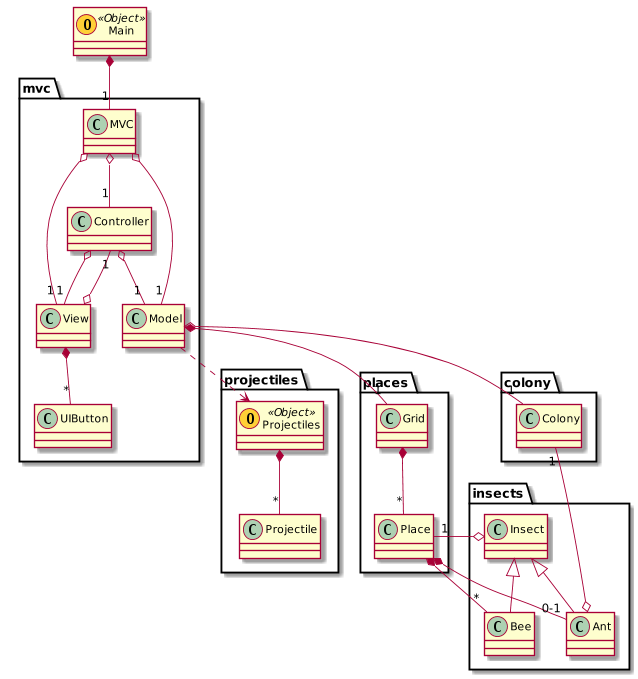
\includegraphics[scale=0.7]{classDiagram.png}
	\caption{Global class UML diagram}
	\label{classDiagram}
\end{figure}
%

	\subsection{Graphic User Interface}
	
	As we have previously said, the GUI, and thus the View part of the MVC, has two roles : %
displaying and warning the Controller of inputs. For the first part, it takes the elements of the game as parameters and draw them, along with the Buttons. %
Secondly, only clicks are used, so there is just to check that the click is on a valid area (i.e. on a Button or on a Place) and then tell the Controller that something has been clicked.
	
	\subsection{Game engine}
	
	As it is turn-based, the game is run by two running timers : one for the frames and a second one for the moves of the insects. %
On each frame (~60 per second) movements are executed, bees move to the right and projectiles get closer to their target. %
On each move (~1 per second) the insects execute their actions like attacking.


\section{Implementation clarifications} % To check, but seems ok

\paragraph{Throwing projectiles} Apart from the instant kill of the Hungry Ants, all attacks are projectiles thrown at the enemy. %
To do that, a target is found by going through the entrances (or exits) of the tunnel, starting by the Place of the insect. %
Once there is a target (if there can possibly be one), a new Projectile is created with a position, a target, and the damages it should inflict on hit.

%
\begin{table}
	\begin{tabular}{c p{8.5cm}}
		\raisebox{-.5\height}{
			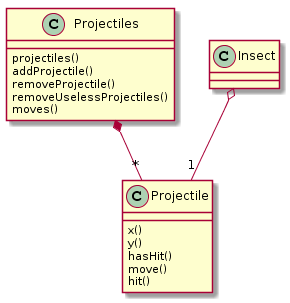
\includegraphics[scale=0.6]{projectileDiagram.png} }
		&
		The constructor of a Projectile consists only on adding itself to list of projectiles of the object Projectiles. %
		After that, on each frame, the object Projectiles is asked to move all of the projectiles. %
		When a Projectile moves it sees if it has touched its target, and if so inflicts damages to the target and puts its field \texttt{hasHit} to true. %
		Later on, Projectiles will be asked to remove the projectiles that have hit their target. \\
	\end{tabular}
\end{table}
%

\paragraph{Bee waves} To deal with the waves, we use a counter to know the wave number. %
The first wave is launched after 6 turns and one wave is launched on each turn from then. %
For that, the Controller part calls the Model function to launch a wave with the level of the bees and the number of the wave as parameters.

%
\begin{table}
	\begin{tabular}{c p{12cm}}
		\raisebox{-.5\height}{
			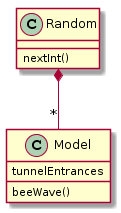
\includegraphics[scale=0.6]{waveDiagram.png} }
		& If the wave number is even, a range bee is launched, a classic bee otherwise. %
		The bee is created with armour points calculated according to the bee level parameter. %
		If the level is high enough, it also has a damage upgrade. We use a random generator to launch the bee in one of the possible tunnel entrances.\\
	\end{tabular}
\end{table}
%

\paragraph{Button menu} The player has the possibility to interact with the game. %
To manage this, we created a class to deal with selection buttons.

%
\begin{figure}[H]
	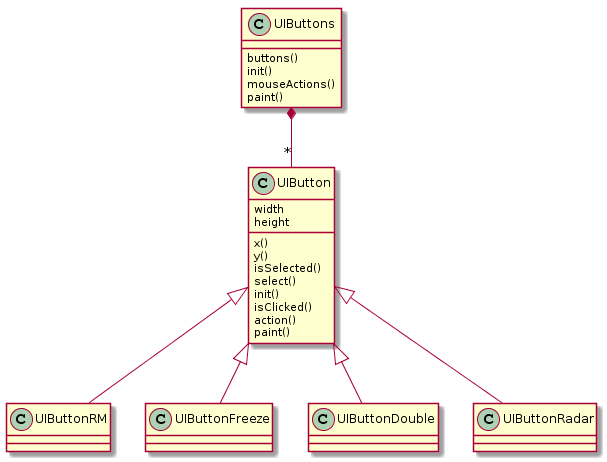
\includegraphics[scale=0.6]{buttonDiagram.png}
\end{figure}
%

Each button has a method to tell if it is being clicked or not. %
If it is, then the action manager in the View part can call the action method of the right button, which then calls the right function in the Model part. %
We also have the possibility to re-initialize the button, because we want at most one button selected at each moment. %
Each button has its method to be drawn. %
We can define new buttons, such as the remove one, or the spells ones, which extend the main button class. %
It is only necessary then to override the definition of the paint and action methods to make it operational. %
Adding a new button to the menu is that way very simple. %
Buttons are gathered in a bigger class, which has a method to deal with the mouse actions. %
This throws a \emph{ClickFound} exception when the click is located, to avoid useless searching.


\paragraph{Information bar} Sometimes, the player is trying to make illegal actions, so it is necessary to display a warning. %
To do this, we created an object \emph{Msg} in View part.

%
\begin{table}
	\begin{tabular}{c p{12cm}}
		\raisebox{-.5\height}{
			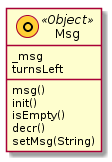
\includegraphics[scale=0.6]{msgDiagram.png} }
		& When a message needs to be displayed, for example when an exception \emph{NotEnoughFood} or \emph{NotEmptyPlace} is caught, we have a method to set a message. %
		It modifies the number of turns left during which the message will be displayed. %
		In the Model part, if the message isn't empty, this number is decreased by one at each turn, and the message is re-initialized when zero is reached.\\
	\end{tabular}
\end{table}
%

\paragraph{Spells} To implement spells, we had to add some fields and methods in the insect and place classes. %
For example, we need boolean fields in the place class to be able to draw an overlay when a place is frozen, or when the ant inside has the radar ability. %
The freeze spell used the same type of counter than the information bar, with a decreasing counter to unfreeze the place after a fixed amount of turns. %
The upgrade spell calls a method to increase the damage power of an insect. %
The radar ability modifies a boolean of all bees in the concerned tunnel, so that the drawing function knows it also has to print the armour points of those bees.


\section{Possible improvements} % To develop more

Along with additions, the existing code can be enhanced. %
To give more than a glimpse of our vision we made a whole section for it.


\paragraph{AI} A possible extension would be to simulate an artificial intelligence, to manage the waves of bees. %
It would know the state of the game, and would choose at each wave the best tunnel to try to exploit the player weaknesses. %
There could also be additional types of bees that counter certain ants and the AI would have to chose the most appropriate.

\paragraph{Better MVC separation and events} For now the MVC isn't perfect as there are visual elements in the code of the Model part. %
For example, bees have their coordinates as fields and move depending on a fixed speed. %
The speed, size of the sprite and that sort of problems belong to the View part. %
Changing this has multiple consequences. How can a bee know if it has reached another Place ? %
How can a projectile know it has hit its target ? %
A solution could be that instead of bees and projectiles checking themselves where they are, they would listen to events that come from de View part. %
The events would be very specific and thus make the code easier to understand. %
Another consequence is that there would be a better modularity and make the management of window size easier.


\section*{Conclusion} % To check, but seems ok

To sum up, we made a tower defence game, using both object-oriented programming and functional programming. %
Our program is organized with a Model-View-Controller separation, and is quite modular. %
Although the structure could be improved, it is at the moment well-organized enough to empower the programmer to add new features easily which is paramount. %
Once that the core of the game is done, it must be simple to add new elements of gameplay, and to modify the graphic user interface. %
We developed our program in this particular intention.


%
\begin{figure}[H]
	
\includegraphics[scale=0.5]{ant_queen.png}
\end{figure}
%

\theEnd

\end{document}